\documentclass[a4paper, 11pt]{article}
	\usepackage[utf8]{inputenc}
    %\usepackage[french]{babel}
    \usepackage[T1]{fontenc}
    \usepackage[top=3cm,, right=2cm,bottom=2cm,left=2cm]{geometry}
    \usepackage{eurosym} %pour le symbole euro

    \usepackage{tabularx}
    \usepackage{soul}
	\usepackage{enumitem}
	\usepackage{pdfpages}
    \usepackage[page]{appendix}
    \renewcommand{\appendixpagename}{Annexes}

    \title{Hackerspace Au Mans}
    \author{Procès-Verbal des Assemblées Générales Ordinaire et Extraordinaire}
    \date{Le jeudi 16 Janvier 2024}

    \newcommand\sep{\noindent\rule{\linewidth}{.5pt}}

    \newcommand{\vote}[5]{

    \smallskip
    \fbox{\begin{minipage}[l]{\textwidth}
    	\smallskip
        \begin{center}
        	\ul{\textsc{Vote}}
        \end{center}

        #1\\
        \textbf{Votants} #2\\
        \textbf{Pour} #3\\
        \textbf{Contre} #4\\
        \textbf{NSPP} #5

        \smallskip

    \end{minipage}}
        \medskip
    }

    \newcommand\question[2]{\noindent\ul{\textit{\textsc{$\bullet$ #1}}}\\#2\\}

    %\ul{#2}}


\begin{document}

\maketitle

\section{Effectifs}

\begin{itemize}
	\item Présents :
		\begin{itemize}
    		\item Jérome Bréhéret
            \item Joel Petit
            \item Manuel Deneu
            \item Romain Bosquet
            \item Sébastien Vallée
            \item Franck Duhil
            \item Romuald Conty
            \item Sébastien Choblet
            \item Laurent Vannier
            \item Florent Touchard
            \item Mathieu Gaborit
            \item Benoit Pau
		\end{itemize}
\end{itemize}

\bigskip

%%La présidence actuelle décide d'accorder le droit de vote à tous les présents pour la durée de cette AG.
\setlist{nosep,after=\vspace{\bigskipamount}}

\section{Assemblée générale ordinaire}
\textbf{La séance est ouverte à 21h30}
\subsection*{Préambule}

Le président lance un vote pour donner droit de vote à l'ensemble des personnes majeures présentes.

\vote{Droit de vote de toutes les personnes majeures présentes}{12}{12}{0}{0}

Le vote est accordé à toutes les personnes majeures présentes dans l'assemblée.

\subsection{Rapport Moral}

Le rapport moral (cf annexe) est présenté par le président.

\vote{Rapport moral}{12}{11}{0}{1}

Le rapport moral est validé par l'assemblée.

\subsection{Rapport Financier}

La trésorière présente le rapport financier (cf annexe).

\vote{Rapport financier}{12}{12}{0}{0}

Le rapport financier est validé par l'assemblée.

\subsubsection{Vie de l'asso : Questions et remarques sur le rapport financier}

Une discution a eu lieu pour évoquer le possible financement d'étagères dans le local 
du HAUM, et constatant la lenteur de ce financement à venir, il est évoqué que ces 
étagères soient financés par le HAUM directement. Il est estimé que cela représenterait 
un cout de 300\euro environ. Cette décision est donc mise au vote.

\vote{Financement en propre des étagères du local}{12}{12}{0}{0}

Les étagères vont donc être financées en propre par l'association.

Une deuxième question porte sur les boîtes qui vont être dans ces étagères, et la question
de financer ces dernières se pose donc et est mise au vote.

\vote{Financement des boîtes "Europe" pour les étagères}{12}{12}{0}{0}

Les boîtes seront donc financées pour remplir les étagères.

\subsection{Élection du bureau}

Afin de faciliter et d'accélérer le vote promulguant les membres du bureau de l'association, 
il est proposé de présenter le même bureau que l'année passée. Aucune contre-indication ne 
vient de l'assemblée à cette annonce.

Se présentent donc à l'élection au bureau :

\begin{itemize}
	\item BREHERET Jérôme
	\item CONTY Romuald
	\item GABORIT Mathieu
	\item TOUCHARD Florent
	\item VALLÉE Sébastien
	\item VANNIER Laurent
\end{itemize}

Il est également convenu avec l'assemblée, toujours dans un but d'accélérer ce vote que ce 
dernier serait voté "en bloc".

La prochaine question mise au vote est donc : "Acceptez vous que la liste précédente soit 
membre du bureau de l'association ?".

\vote{Élection des membres du bureau}{12}{12}{0}{0}

\textbf{La séance est levée à 22h20}

\section{Réunion de bureau}

Alors que l'ensemble des membres du nouveau bureau est présent, il est décidé de procéder 
dans l'immédiat aux élections internes à celui-ci. Pour les votes suivants, le collège 
électoral est réduit au bureau seul (soit 6 membres). Afin d'accélerer le vote, il est
décidé de voter pour que chaque personne soit reconduit dans son role au sein du bureau, 
les membres de celui-ci n'ayant pas changé.

Le vote concerne donc l'attribution de ces postes :
\begin{itemize}
    \item Jérôme BRÉHERET au poste de président
    \item Mathieu GABORIT au poste de trésorier
    \item Florent TOUCHARD au poste de vice-trésorier
    \item Sébastien VALLÉE au poste de secrétaire
    \item Laurent VANNIER au poste de vice-secrétaire
\end{itemize}

\vote{Reconduction des roles au sein du bureau}{6}{6}{0}{0}

Le bureau est donc reconduit parfaitement.

\section{Composition du bureau}
\begin{description}
  \item[Président] Jérôme BRÉHÉRET
  \item[Trésorier] Mathieu GABORIT
  \item[Vice-Trésorier] Florent TOUCHARD
  \item[Secrétaire] Sébastien VALLÉE
  \item[Vice-Secrétaire] Laurent VANNIER
  \item[Membre du bureau] Romuald CONTY
\end{description}

La composition du bureau est validé par l'assemblée.
\bigskip

\textbf{La séance est levée à 22h30.}

\bigskip\bigskip

\sep

\bigskip\bigskip

Le présent procès-verbal est approuvé par le président du HAUM.

\bigskip\bigskip

Président :



\clearpage
\begin{appendices}
\section{Rapport Moral}

\subsection{Vie de l'association}

Le nombre d'adhérents réaugmente régulièrement depuis la fin de l'épidémie de Covid et en
2023, le HAUM a enregistré 21 cotisations dont 2 entreprises.
Depuis Août 2022 nous utilisons HelloAsso pour permettre le paiement des cotisations en ligne.

\subsection{Bilan}

\subsubsection{Le Mans Innovation}

Suite au déménagement en 2017, le HAUM a largement investi le nouveau local. L'association dispose d'un atelier propre et d'un atelier sale. Ce dernier a bénéficié d'un grand ménage lors de l'installation d'une entreprise dans les locaux de LMI. Aujourd'hui la tenue globale est correcte mais il faut veiller à ne pas en refaire un lieu de dépot. 

Grâce à un don de l'Université du Mans, le local s'est équipé en mobilier, notamment en tables et établis et des discussions sont actuellement en cours avec Le Mans Innovation pour installer une zone de stockage sur étagères. 

Il est important de mettre en place un roulement pour le rangement du HAUM et maintenir le local dans un état utilisable.

\subsubsection{Évènements}

Depuis la dernière AG (en août 2022), Le HAUM a participé à de nombreux évènements et proposé autant de
projets innovants présentés succinctement ci-après.

\paragraph{Teriaki 2022} Morpion 3D qui n'a malheureusement pas marché suite à un problème technique.

\paragraph{Digital ON} Octobre 2022 pour un public pas très nombreux mais curieux du projet présenté. Cet évènement a d'ailleurs permis de fiabiliser le Morpion 3D présenté en août.

\paragraph{Les 24heures du code} Le projet Vrhaum, basé sur des voitures radiocommandées modifiées et augmentées a permis aux participants de construire une interface autour de nos logiciels et se mesurer sur un circuit long d'une soixantaine de mètres. Ce sujet ambitieux avec une belle implication des membres du HAUM. Les concourants et les autres organisateurs ont apprécié aussi bien le coté technique que le coté jeu de ce sujet.

\paragraph{Teriaki 2023} Le projet HAUMogramme, une table-séquenceur circulaire permettant au public de créer de la musique en déplaçant physiquement des marqueurs, a été très bien reçu.

\paragraph{Barbecue d'automne} Moment convivial autour d'un barbecue en plein mois de novembre sous la serre d'un des membres.
%a l'abri sous la serre de notre amis Nugets, la prochaine foi on s'arrangera pour pouvoir essayer la pelleteuse 

\paragraph{Les sessions bidouille} Chaque mardi soir les portes du HAUM sont ouvertes à tout ceux et celles qui veulent bien les pousser.

\subsubsection{Projets et axes}

Il y a plusieurs projets en cours. Au niveau collectif (pour des projets qui occupent
quelques personnes) on a aujourd'hui:

\begin{description}
	\item[Photographie] Sténopé, stéréo-photographie, etc\ldots
    \item[HAUMogramme] Installation sonore (et lumineuse ?)
	\item[IdiHAUM\footnotemark]\footnotetext{Nom non définitif} Solution de contrôle d'accès
\end{description}

Les réunions "projets" qui avaient été proposées et instaurées lors de la dernière année
ont été plutôt bien suivies et utiles au début de l'exercice et ont complètement disparu
pendant l'été. Elle permettaient à tous de s'informer des projets en cours régulièrement
elle sont à relancer et pourraient êtres couplées à des annonces sur le forum.

\subsection{Matériel disponible}

Le HAUM dispose actuellement du matériel suivant (entre autres):

\begin{description}
    \item Une découpeuse laser (Pret de Le Mans Innovation)
    \item Une imprimante 3D (Pret de Le Mans Innovation)
    \item Une découpeuse vinyle Caméo (plotter de découpe)
    \item Outils pour l'électronique (dont un fer à souder acquis par le HAUM cette année)
    \item Outillage électroportatif et manuel
    \item Fraiseuse CNC 3 axes de table
    \item La majorité des projets passés
\end{description}

\section{Rapport Financier}
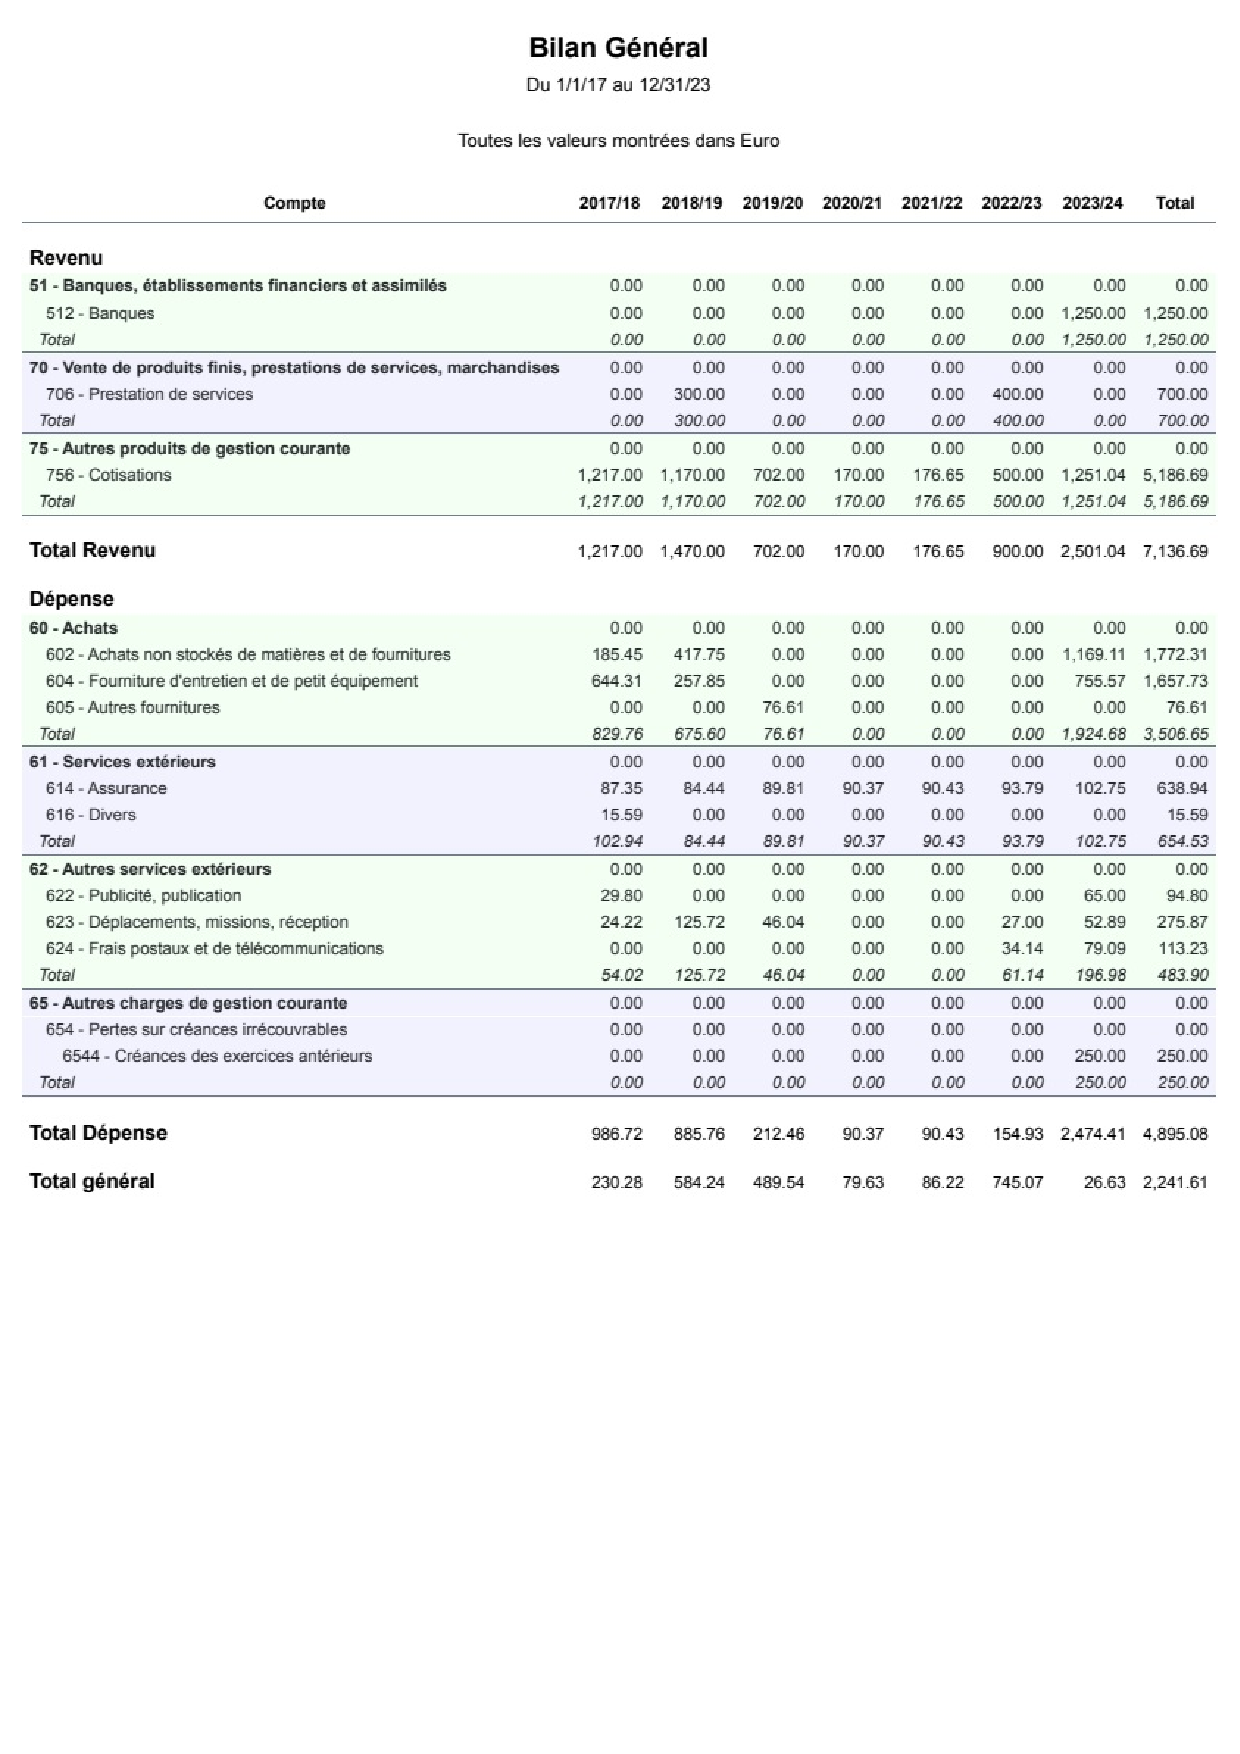
\includegraphics[scale=0.9]{../convocation/bilan2023_general.pdf}
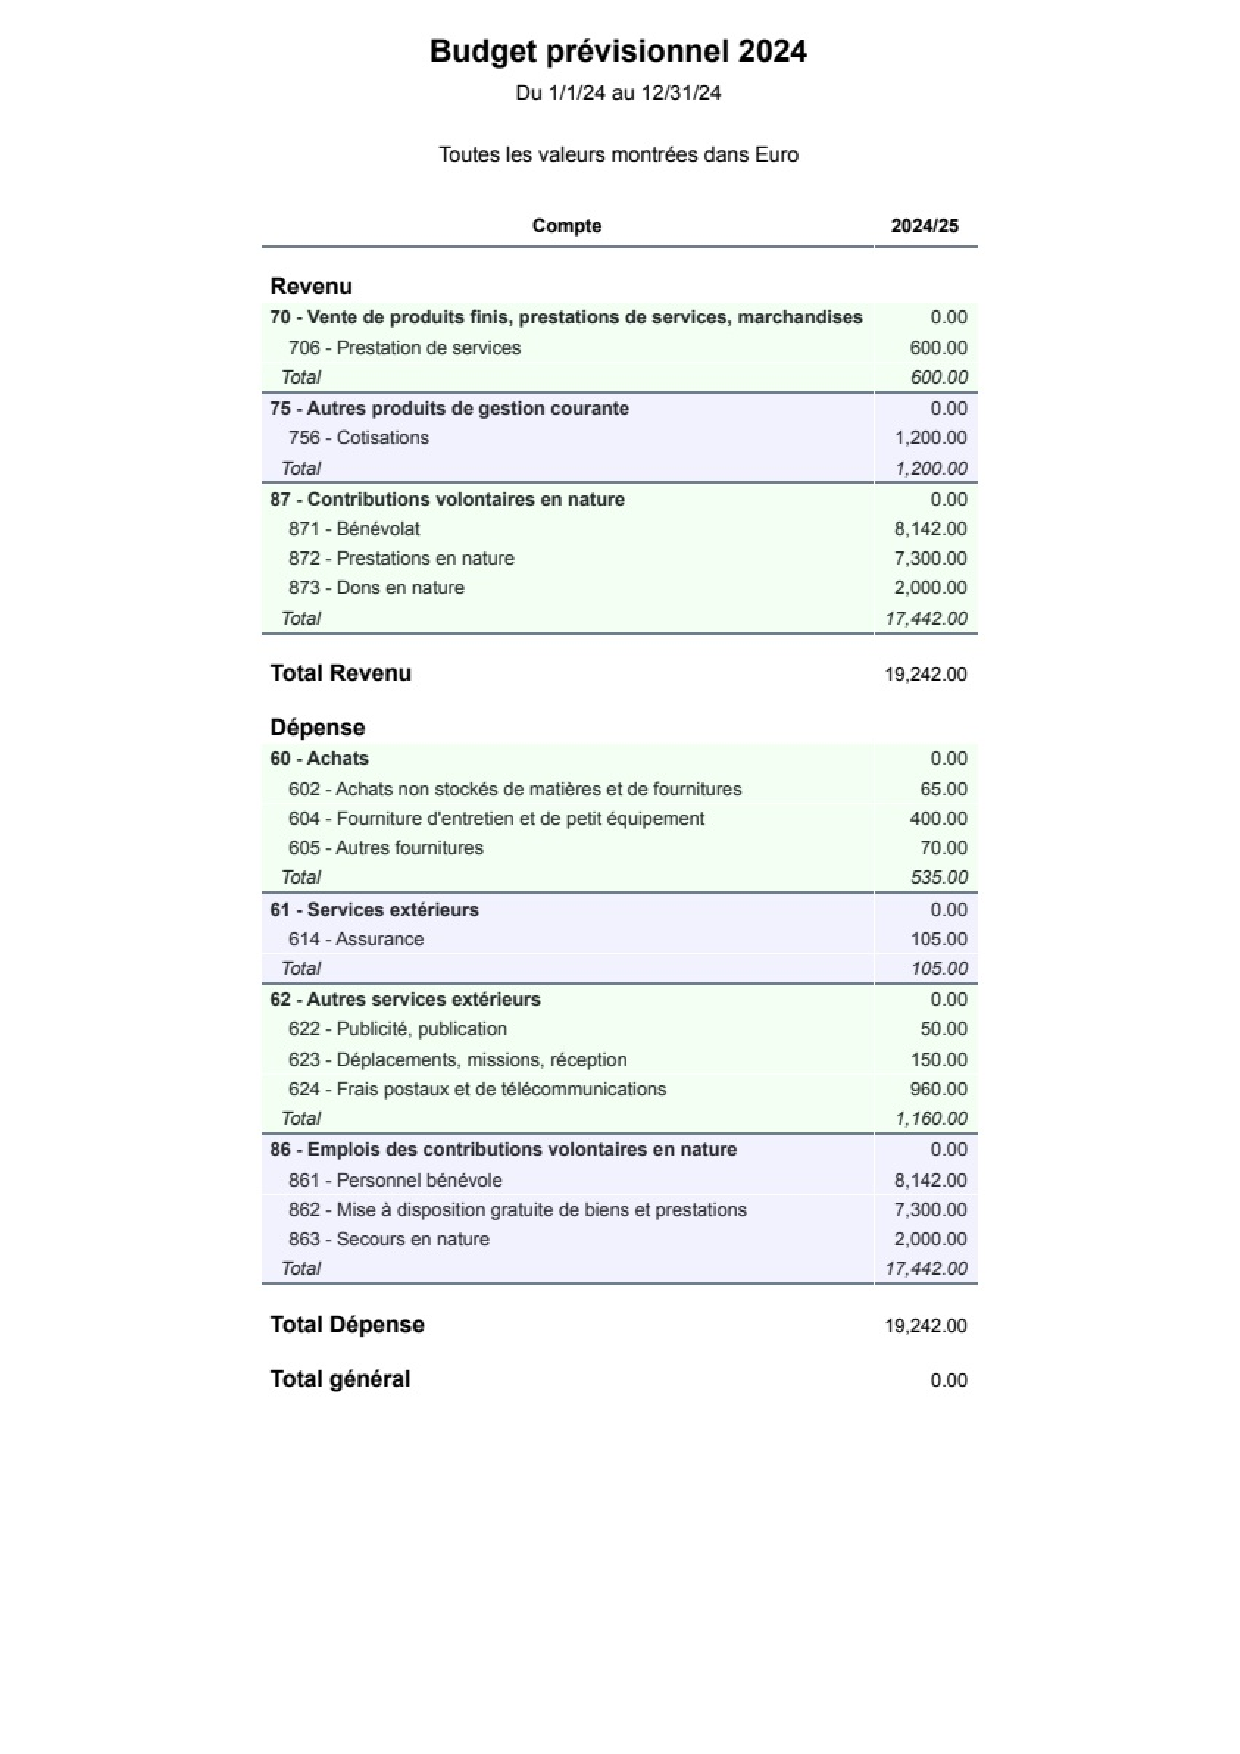
\includepdf[pages=-]{../convocation/prev2024.pdf}
